

\usepackage{graphicx}
\DeclareGraphicsExtensions{.pdf,.png}
\usepackage{url}
\usepackage{ragged2e}
\usepackage{times}
\usepackage{array}
\usepackage{amsmath}
\usepackage{amssymb}
\usepackage{caption}
\usepackage{subcaption}
\usepackage[inline]{enumitem}
\usepackage{float}
\usepackage{xcolor}
\usepackage{colortbl}
\usepackage{makecell}
\usepackage{xspace}
\usepackage{etoolbox}
\usepackage{tikz}
\DeclareMathOperator*{\argmax}{arg\,max}

\newcommand{\R}{\mathbb{R}}
\newcommand{\SUM}{\emph{SH}}
\newcommand{\MAX}{\emph{MH}}

\newcommand{\OC}{\emph{1C}}
\newcommand{\TC}{\emph{10C}}
\newcommand{\RC}{\emph{RC}}
\newcommand{\TCV}{\emph{10C+rV}}
\newcommand{\RCV}{\emph{RC+rV}}
\newcommand{\RV}{\emph{rV}}

\newcommand{\order}{\emph{Order}}
\newcommand{\orderz}{\emph{Order0}}
\newcommand{\orderpp}{\emph{Order++}}
\newcommand{\VSE}{\emph{UVS}}
\newcommand{\VSEpp}{\emph{VSE++}}
\newcommand{\VSEppFt}{\emph{VSE++ (FT)}}
\newcommand{\VSEppRes}{\emph{VSE++ (ResNet)}}
\newcommand{\VSEppResFt}{\emph{VSE++ (ResNet, FT)}}
\newcommand{\VSEz}{\emph{VSE0}}
\newcommand{\VSEzFt}{\emph{VSE0 (FT)}}
\newcommand{\VSEzRes}{\emph{VSE0 (ResNet)}}
\newcommand{\VSEzResFt}{\emph{VSE0 (ResNet, FT)}}




\newcommand{\coco}{MS-COCO}
\newcommand{\fthk}{Flickr30K}
 
\newcommand{\T}{\ensuremath{\top}} 
\captionsetup[subfigure]{subrefformat=simple,labelformat=simple}
\renewcommand\thesubfigure{(\alph{subfigure})}


\newcounter{rowcntr}[table]
\renewcommand{\therowcntr}{\the\numexpr\thetable+1.\arabic{rowcntr}}

\newcommand{\numrow}{\refstepcounter{rowcntr}\therowcntr}

\AtBeginEnvironment{tabular}{\setcounter{rowcntr}{0}}

\newcolumntype{H}{>{\setbox0=\hbox\bgroup}c<{\egroup}@{}}

\newcommand{\comment}[1]{}
\makeatletter
\def\blfootnote{\gdef\@thefnmark{}\@footnotetext}
\makeatother


\newcommand{\FF}[1]{{\color{blue}{[Fartash: #1]}}}
\newcommand{\JK}[1]{{\color{purple}{[Jamie: #1]}}}
\newcommand{\DF}[1]{{\color{cyan}{[David: #1]}}}
\newcommand{\SF}[1]{{\color{red}{[Sanja: #1]}}}




\title{VSE++: Improving Visual-Semantic
Embeddings with Hard Negatives}

\addauthor{Fartash Faghri}{faghri@cs.toronto.edu}{1}
\addauthor{David J. Fleet}{fleet@cs.toronto.edu}{1}
\addauthor{Jamie Ryan Kiros}{kiros@google.com}{2}
\addauthor{Sanja Fidler}{fidler@cs.toronto.edu}{1}

\addinstitution{Department of Computer Science,\\
University of Toronto \\
and\\
Vector Institute
}
\addinstitution{Google Brain Toronto
}

\runninghead{Faghri \etal}{VSE++: Improving Visual-Semantic Embeddings with H.  
N.}

\def\eg{\emph{e.g}\bmvaOneDot}
\def\Eg{\emph{E.g}\bmvaOneDot}
\def\etal{\emph{et al}\bmvaOneDot}

\begin{document}

\maketitle

\vspace{-1mm}
\begin{abstract}
    We present a new technique for learning visual-semantic embeddings for 
    cross-modal retrieval.  Inspired by hard negative mining, the use of hard 
    negatives in structured prediction, and ranking loss functions, we 
    introduce a simple change to common loss functions used for multi-modal 
    embeddings.  That, combined with fine-tuning and use of augmented data, 
    yields significant gains in retrieval performance.  We showcase our 
    approach, \VSEpp, on \coco{} and \fthk{} datasets, using ablation studies 
    and comparisons with existing methods.  On \coco{} our approach outperforms 
    state-of-the-art methods by  in caption retrieval and  in 
    image retrieval (at R@).\blfootnote{Work done while a Ph.D. student 
    at the University of Toronto.}
\end{abstract}

\section{Introduction}

Joint embeddings enable a wide range of tasks in image, video and language 
understanding. Examples include shape-image embeddings (\cite{li2015joint}) 
for shape inference, bilingual word embeddings (\cite{zou2013bilingual}), 
human pose-image embeddings for 3D pose inference (\cite{li2015maximum}), 
fine-grained recognition (\cite{reed2016learning}), zero-shot learning 
(\cite{frome2013devise}), and modality conversion via synthesis 
(\cite{reed2016generative,reed2016learning}).  Such embeddings entail 
mappings from two (or more) domains into a common vector space in 
which semantically associated inputs (e.g., text and images) are mapped to 
similar locations.  The embedding space thus represents the underlying 
domain structure, where location and often direction are 
semantically meaningful.

{\em Visual-semantic embeddings} have been central to
image-caption retrieval and 
generation~\cite{kiros2014unifying,karpathy2015deep}, and visual 
question-answering~\cite{Malinowski15}.  One approach to visual 
question-answering, for example, is to first describe an image by a set of 
captions, and then to find the nearest caption in response to a question 
(\cite{agrawal2017vqa,zitnick2016measuring}). For image synthesis 
from text, one could map from text to the joint embedding space, and then
back to image space (\cite{reed2016generative,reed2016learning}).

Here we focus on visual-semantic embeddings for cross-modal retrieval; 
i.e.\ the retrieval of images given captions, 
or of captions for a query image.  As is common in retrieval, 
we measure performance by R@, i.e., recall at  -- the fraction of 
queries for which the correct item is retrieved in the closest  points 
to the query in the embedding space ( is usually a small integer, 
often ).  More generally, retrieval is a natural way to assess the 
quality of joint embeddings for image and language data (\cite{hodosh2013framing}).

The basic problem is one of ranking; the correct target(s) 
should be closer to the query than other items in the corpus, not unlike
{\em learning to rank}\/ problems (e.g., \cite{li2014learning}), and 
max-margin structured prediction \cite{chapelle2007large,le2007direct}.
The formulation and model architecture in this paper are most closely 
related to those of \cite{kiros2014unifying}, learned with a triplet ranking 
loss.  In contrast to that work, we advocate a novel loss, the use of 
augmented data, and fine-tuning, which, together, produce a significant 
increase in caption retrieval performance over the baseline ranking loss on 
well-known benchmark data.  We outperform the best reported result on 
\coco{} by almost .  We also show that the benefit of a more 
powerful image encoder, with fine-tuning, is amplified with 
the use of our stronger loss function.
We refer to our model as \VSEpp{}.
To ensure reproducibility, our code is publicly 
available~\footnote{\url{https://github.com/fartashf/vsepp}}.

Our main contribution is to incorporate hard negatives in the loss 
function.  This was inspired by the use of hard negative mining in 
classification tasks (\cite{dalal2005histograms, 
felzenszwalb2010object, malisiewicz2011ensemble}), and by the use of
hard negatives for improving image embeddings for face recognition 
(\cite{schroff2015facenet, wu2017sampling}). Minimizing a loss function using 
hard negative mining is equivalent to minimizing a modified non-transparent 
loss function with uniform sampling.  We extend the idea with the explicit 
introduction of hard negatives in the loss for multi-modal embeddings, 
without any additional cost of mining.

We also note that our formulation complements other recent articles that 
propose new architectures or similarity functions for this problem. To this 
end, we demonstrate improvements to \cite{vendrov2015order}.
Among other methods that could be improved with a modified loss, 
\cite{wang2017learning} propose an embedding network to fully 
replace the similarity function used for the ranking loss.  An attention 
mechanism on both images and captions is used by \cite{nam2016dual}, where the 
authors sequentially and selectively focus on a subset of words and image 
regions to compute the similarity.  In \cite{huang2016instance}, the authors 
use a multi-modal context-modulated attention mechanism to compute the 
similarity between images and captions. Our proposed loss function and 
triplet sampling could be extended and applied to other such problems.




\comment{word-image embeddings (\cite{weston2010large}).
    Other examples are grounding phrases and semantics (\cite{xiao2017weakly}, 
    \cite{baroni2016grounding}) and object retrieval.  \fartash{TODO: Natural 
    Language Object Retrieval, Learning what and where to draw, Measuring 
    machine intelligence through visual question answering, Weakly-supervised 
    Visual Grounding of Phrases with Linguistic Structures, Grounding 
    distributional semantics in the visual world}}

\comment{{{.
In this paper, we advocate loss functions that directly improve the retrieval 
performance. When recall performance at  (R@) is high, there is a higher 
probability that the first retrieved result is a correct match.  Consequently, 
less computation is needed for retrieving more items and further re-ranking.  

A triplet loss over a triplet of anchor, positive and negative examples is 
defined as a hinge loss that penalizes the model for the negative example being 
a better match to the anchor than the positive example.  Previous work sum over 
the loss for all triplets or a random sample of triplets for mini-batch 
optimization algorithms.  In \cite{frome2007learning}, the authors considered 
pruning the possible set of triplets\fartash{should either remove this or 
expand it}.

To the best of our knowledge, combining the idea of hard negatives with 
mini-batch training has not been done before. 

Older work (\cite{Lin:2014db}) performed matching between words and objects 
based on classification scores.

Our results on \coco{} show a dramatic increase in caption retrieval 
performance over the baseline. The new loss function alone outperforms the 
baseline by . With all introduced changes, \VSEpp{} achieves an absolute 
improvement of  in R@1, which corresponds to a  relative 
improvement. We outperform the best reported result on \coco{} by almost .  
To ensure reproducibility, our code is publicly 
available~\footnote{\url{https://github.com/fartashf/vsepp}}.

We refer to our model as \VSEpp{}. Our loss function and architecture is mostly 
related to the visual-semantic embeddings of \cite{kiros2014unifying} which we 
refer to as \VSE{}.

We also demonstrate the importance of using more powerful image encoders and 
fine-tuning the image encoder. We achieve further improvements exploiting more 
data, and employing a multi-crop trick from \cite{klein2015associating}.  Our 
results on \coco{} show a dramatic increase in caption retrieval performance 
over \VSE{}. The new loss function alone outperforms the original model by 
. With all introduced changes, \VSEpp{} achieves an absolute improvement 
of  in R@1, which corresponds to a  relative improvement. We 
outperform the best reported result on \coco{} by almost .  To ensure 
reproducibility, our code is publicly 
available~\footnote{\url{https://github.com/fartashf/vsepp}}.
}}}
 \vspace{-3mm}
\section{Learning Visual-Semantic Embeddings}



For image-caption retrieval the query is a caption and the task is to 
retrieve the most relevant image(s) from a database. Alternatively, the 
query may 
be an image, and the task is to retrieves relevant captions.  The goal is to 
maximize recall at  (R@), i.e., the fraction of queries for which the 
most relevant item is ranked among the top  items returned.

Let  be a training set of image-caption pairs.  
We refer to  as {\em positive pairs}\/ and  as 
{\em negative pairs}\/; i.e., the most relevant caption to the image  is 
 and for caption , it is the image .  We define a similarity 
function  that should, ideally, give higher similarity 
scores to positive pairs than negatives.  In caption retrieval, the query 
is an image and we rank a database of captions based on the similarity 
function; i.e., R@ is the percentage of queries for which the positive 
caption is ranked among the top  captions using .  Likewise 
for image retrieval.  In what follows the similarity function is defined 
on the joint embedding space.  This differs from other formulations, such 
as \cite{wang2017learning}, which use a similarity network to directly 
classify an image-caption pair as matching or non-matching.

\vspace{-3mm}
\subsection{Visual-Semantic Embedding}

Let  be a feature-based representation 
computed from image  (e.g.\ the representation before logits in 
VGG19~(\cite{simonyan2014very}) or ResNet152~(\cite{he2016deep})).  
Similarly, let  be a representation
of caption  in a caption embedding space (e.g.\ a GRU-based text 
encoder).  Here,  and  denote model 
parameters for the respective mappings to these initial 
image and caption representations.

Then, let the mappings into the {\em joint embedding space}\/ 
be defined by linear projections:

where  and .
We further normalize , and , 
to lie on the unit hypersphere.  Finally, we define the similarity 
function in the joint embedding space to be the usual inner product:

Let  be the model parameters.  If we also
fine-tune the image encoder, then we would also include  in 
.

Training entails the minimization of empirical loss with respect to , 
i.e., the cumulative loss over training data :

where  is a suitable loss function for a single training 
exemplar.
Inspired by the use of a triplet loss for image retrieval
(e.g., \cite{frome2007learning,chechik2010large}), recent approaches
to joint visual-semantic embeddings have used a hinge-based triplet ranking 
loss \cite{kiros2014unifying, karpathy2015deep, ZhuICCV15, 
socher2014grounded}:

where  serves as a margin parameter, and .  
This hinge loss comprises two symmetric terms.  The first sum is taken over all 
negative captions , given query .  The second is taken over all 
negative images , given caption .  Each term is proportional to the 
expected loss (or {\em violation}\/) over sets of negative samples.  If  and 
 are closer to one another in the joint embedding space than to any 
negative, by the margin , the hinge loss is zero.  In practice, for 
computational efficiency, rather than summing over all  negatives in the 
training set, it is common to only sum over (or randomly sample) the negatives 
in a mini-batch of stochastic gradient descent \cite{kiros2014unifying, 
socher2014grounded, karpathy2015deep}.  The runtime complexity of computing 
this loss approximation is quadratic in the number of image-caption pairs in 
a mini-batch.

Of course there are other loss functions that one might consider.
One  is a pairwise hinge loss in which elements of positive pairs
are encouraged to lie within a hypersphere of radius  in 
the joint embedding space,
while negative pairs should be no closer than .
This is problematic as it constrains the structure of the latent space more 
than does the ranking loss, and it entails the use of two hyper-parameters 
which can be very difficult to set.
Another possible approach is to use Canonical Correlation Analysis to learn 
 and , thereby trying to preserve correlation between the text and 
images in the joint embedding (e.g., 
\cite{klein2015associating,eisenschtat2016linking}).  By comparison, when 
measuring performance as R@, for small , a correlation-based loss will 
not give sufficient influence to the embedding of negative items in the local 
vicinity of positive pairs, which is critical for R@.  

\subsection{Emphasis on Hard Negatives}
\label{sec:hard_neg}

\begin{figure*}[t!]

\hspace*{-1cm}
    \centering
    \def\xx{5}
    \def\rr{1.5}
    \def\nn{.5}
    \begin{subfigure}[b]{.18\textwidth}
        \hspace*{-.6cm}
        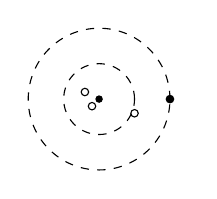
\begin{tikzpicture}[scale=0.9]
            \draw[dashed] (0, 0) circle (\rr);
            \fill (0,0) circle (1.5pt) node[left] {};
            \fill (\rr,0) circle (1.5pt) node[right] {};
            \draw[dashed] (0, 0) circle (.5);
            \draw (+\nn,0) circle (1.5pt) node[right] {};



            \draw (-.1,\rr-.1) circle (1.5pt) node[above] {};
            \draw (+-\rr+.2,+.1) circle (1.5pt) node[left] {};
            \draw (0.5,-\rr+.2) circle (1.5pt) node[below] {};
        \end{tikzpicture}
        \caption{}\label{fig:hardneg}
    \end{subfigure}
\hspace*{2cm}
    \begin{subfigure}[b]{.18\textwidth}
        \hspace*{-.6cm}
        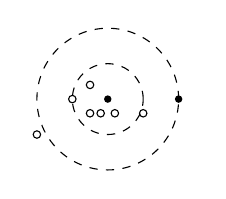
\begin{tikzpicture}[scale=0.9]
            \draw[dashed] (0, 0) circle (\rr);
            \fill (0,0) circle (1.5pt) node[left] {};
            \fill (\rr,0) circle (1.5pt) node[right] {};
            \draw[dashed] (0, 0) circle (.5);
            \draw (\rr-.5,0) circle (1.5pt) node[right] {};

            \draw (-.1,\rr-.1-.1) circle (1.5pt) node[above] {};
            \draw (-\rr+.25,+.2) circle (1.5pt) node[left] {};
            \draw (0.5,-\rr+.2) circle (1.5pt) node[below] {};
            \draw (-1.,\rr-.5) circle (1.5pt) node[above] {};
            \draw (-\rr+.25,-.2) circle (1.5pt) node[left] {};
            \draw (0.1,-\rr+.2) circle (1.5pt) node[below] {};
        \end{tikzpicture}
        \captionsetup{margin=.5cm}
        \caption{}\label{fig:softneg}
    \end{subfigure}
    \caption{\small An illustration of typical positive pairs and the nearest negative 
    samples. Here assume similarity score is the negative distance. Filled 
    circles show a positive pair , while empty circles are negative 
    samples for the query .  The dashed circles on the two sides are drawn 
    at the same radii.  Notice that the hardest negative sample  is 
    closer to  in \subref{fig:hardneg}. Assuming a zero margin, 
    \subref{fig:softneg} has a higher loss with the \SUM{} loss compared to 
    \subref{fig:hardneg}.  The \MAX{} loss assigns a higher loss to 
    \subref{fig:hardneg}.}
    \label{fig:examples}
\end{figure*}
 
Inspired by common loss functions used in structured prediction 
(\cite{tsochantaridis2005large, yu2009learning, felzenszwalb2010object}), we 
focus on hard negatives for training, i.e., the negatives closest to each 
training query.  This is particularly relevant for retrieval since it is the 
hardest negative that determines success or failure as measured by R@.  




Given a positive pair , the hardest negatives are given by 
 and .
To emphasize hard negatives we define our loss as

Like Eq.~\ref{eq:contrastive}, this loss comprises two terms, 
one with  and one with  as queries.  Unlike Eq.~\ref{eq:contrastive}, 
this loss is specified in terms of the hardest negatives,   and 
. We refer to the loss in Eq.~\ref{eq:rank_loss} 
as {\em Max of Hinges (\MAX{})}\/ loss, and the loss in 
Eq.~\ref{eq:contrastive} as {\em Sum of Hinges (\SUM{})}\/ loss. There is 
a spectrum of loss functions from the \SUM{} loss to the \MAX{} loss. In the 
\MAX{} loss, the winner takes all the gradients, where instead we use 
re-weighted gradients of all the triplets. We only discuss the \MAX{} loss as 
it was empirically found to perform the best.

One case in which the \MAX{} loss is superior to \SUM{} is when multiple 
negatives with small violations combine to dominate the \SUM{} loss.  
For example, Fig.~\ref{fig:examples} depicts a positive pair
together with two sets of negatives.  In Fig.~\ref{fig:hardneg}, a 
single negative is too close to the query, which may require
a significant change to the mapping.  
However, any training step that pushes the hard negative 
away, might cause a number of small violating negatives, as 
in Fig.~\ref{fig:softneg}. Using the \SUM{} loss, these `new' negatives 
may dominate the loss, so the model is pushed back to the first 
example in Fig.~\ref{fig:hardneg}.  This may create local minima in the 
\SUM{} loss that may not be as problematic for the \MAX{} loss, which focuses
on the hardest negative.

For computational efficiency, instead of finding the hardest negatives in the 
entire training set, we find them within each mini-batch.  
This has the same quadratic 
complexity as the complexity of the \SUM{} loss.  With random 
sampling of the mini-batches, this approximation yields other advantages.  One is 
that there is a high probability of getting hard negatives that are harder than 
at least  of the entire training set.  Moreover, the loss is potentially 
robust to label errors in the training data because the probability of sampling 
the hardest negative over the entire training set is somewhat low.









\subsection{Probability of Sampling the Hardest Negative}
\label{sec:prob_hard_neg}

Let  denote a training set of image-caption pairs,
and let  denote the set of captions.  Suppose we draw  samples 
in a mini-batch, , from .  Let the permutation, 
, on  refer to the rankings of captions according to the similarity 
function  for . We can assume 
permutations, , are uncorrelated.

Given a query image, , we are interested in the probability of getting 
no captions from the th percentile of  in the mini-batch. 
Assuming IID samples, this probability is simply , the probability 
that no sample in the mini-batch is from the th percentile. 
This probability tends to zero exponentially fast, falling below  
for . Hence, for large enough mini-batchs, with high probability 
we sample negative captions that are harder 
than  of the entire training set.
The probability for the th percentile of  tends to zero 
more slowly; it falls below  for , which is a relatively 
large mini-batch. 

While we get strong signals  by randomly 
sampling negatives within mini-batches, such sampling also provides 
some robustness to outliers, such as negative captions that 
better describe an image compared to the ground-truth caption.
Mini-batches as small as  can provide strong 
enough training signal and robustness to label errors. Of course by 
increasing the mini-batch size, we get harder negative examples and possibly 
a stronger training signal.  However, by increasing the mini-batch size, we lose 
the benefit of SGD in finding good optima and exploiting the gradient noise.  
This can lead to getting stuck in local optima or as observed by 
\cite{schroff2015facenet}, extremely long training time.





 \section{Experiments}

\begin{table*}[t!]
\resizebox{\linewidth}{!}{
    \centering
     \begin{tabular}{c|c|c|HccccH|ccccH}
         \# &
         {\bf Model} & {\bf Trainset} & {\bf R Sum}
         & \multicolumn{5}{c|}{Caption Retrieval}
         & \multicolumn{5}{c}{Image Retrieval}\\
         & & & &
         {\bf R@1} & {\bf R@5} & {\bf R@10} & {\bf Med r} & {\bf Mean r} &
         {\bf R@1} & {\bf R@5} & {\bf R@10} & {\bf Med r} & {\bf Mean r}\\
         \hline
         & & \multicolumn{12}{c}{{\cellcolor[gray]{0.8}\bf 1K Test Images}}\\
         \hline
\numrow{}\label{coco:VSE}&
         \VSE{}~(\cite{kiros2014unifying}, GitHub) & \OC{} (1 fold) &
          &
          &  &  &  & - &
          &  &  &  & - \\
         \numrow{} &
         \order{}~(\cite{vendrov2015order})& \TCV{} &
         - &
          & - &  &  &  &
          & - &  &  & \\
         \numrow{} &
         Embedding Net~(\cite{wang2017learning}) & \TCV{} &
         - &
          &  &  & - & - &
          &  &  & - & -
         \\
         \numrow{}\label{coco:smLSTM} &
         sm-LSTM~(\cite{huang2016instance}) &? &
          &
          &  &  &  & - &
          &  &  &  & -
         \\
         \numrow{}\label{coco:twoway} &
         2WayNet~(\cite{eisenschtat2016linking}) & \TCV{} &
         - &
          &  & - & - & - &
          &  & - & - & -
         \\
         \hline
\numrow{}\label{coco:VSEppOC} &
         \VSEpp{} & \OC{} (1 fold) &
          &
          &  &  &  &  &
          &  &  &  & \\

\numrow{}\label{coco:VSEppRC} &
         \VSEpp{} & \RC &
          &
          &  &  &  &  &
          &  &  &  & \\


\numrow{}\label{coco:VSEppRCV} &
         \VSEpp{} & \RCV{} &
          &
          &  &  &  &  &
          &  &  &  & \\

\numrow{}\label{coco:VSEppFt} &
         \VSEppFt{} & \RCV{} &
          &
          &  &  &  &  &
          &  &  &  & \\

\numrow{}\label{coco:VSEppRes} &
         \VSEppRes{} & \RCV{} &
          &
          &  &  &  &  &
          &  &  &  & 
         \\

\numrow{}\label{coco:VSEppResFt} &
         \VSEppResFt{} & \RCV{} &
          &
          &  &  &  
         &  &
          &  &  &  
         & 
         \\

        \hline
         & & \multicolumn{12}{c}{{\cellcolor[gray]{0.8}\bf 5K Test Images}}\\
         \hline
         \numrow{} &
         \order{}~(\cite{vendrov2015order})& \TCV{} &
         - &
          & - &  &  &  &
          & - &  &  & \\

\numrow{}\label{coco:VSEppFt5} &
         \VSEppFt{} & \RCV{} &
          &
          &  &  &  &  &
          &  &  &  & \\

\numrow{}\label{coco:VSEppResFt5} &
         \VSEppResFt{} & \RCV{} &
          &
          &  &  &  
         &  &
          &  &  &  
         & 
        \-1mm]

\end{tabular}
    }
    \vspace{.2cm}
    \caption{\small The effect of data augmentation and fine-tuning. We copy the 
    relevant results for \VSEpp{} from Table~\ref{tb:coco} to enable an easier 
    comparison.  Notice that after applying all the modifications, \VSEz{} 
    model reaches  for , while \VSEpp{} achieves .}
    \label{tb:vse0}
    \vspace{-.4cm}
 \end{table*}

The results on the \coco{} dataset are presented in Table~\ref{tb:coco}.  To 
understand the effect of training and algorithmic variations we report ablation 
studies for the baseline \VSEz{} (see Table~\ref{tb:vse0}).  Our best result 
with \VSEpp{} is achieved by using ResNet152 and fine-tuning the image encoder 
(row~\ref{coco:VSEppResFt}), where we see  improvement in R@1 for 
caption retrieval and  improvement in R@1 for image retrieval compared to 
\VSE{} (rows~\ref{coco:VSE} and~\ref{coco:VSEppResFt}).  Notice that using 
ResNet152 and fine-tuning can only lead to  improvement using the 
\VSEz{} formulation (rows~\ref{coco:VSEzResFt} and~\ref{coco:VSE}), while our 
\MAX{} loss function brings a significant gain of  
(rows~\ref{coco:VSEppResFt} and~\ref{coco:VSEzResFt}).



Comparing \VSEppResFt{} to the current state-of-the-art on \coco{}, {\em 
2WayNet}\/ (row~\ref{coco:VSEppResFt} and row~\ref{coco:twoway}), we see 
 improvement in R@1 for caption retrieval and compared to 
{\em sm-LSTM}\/ (row~\ref{coco:VSEppResFt} and row~\ref{coco:smLSTM}), 
 improvement in image retrieval.
We also report results on the full  test set of \coco{} in 
rows~\ref{coco:VSEppFt5} and~\ref{coco:VSEppResFt5}.

\emph{Effect of the training set}. We compare \VSEz{} and \VSEpp{} by 
incrementally improving the training data.  Comparing the models trained on 
\OC{} (rows~\ref{coco:VSE} and~\ref{coco:VSEppOC}), we only see  
improvement in R@1 for image retrieval but no improvement in caption retrieval 
performance. However, when we train using \RC{} (rows~\ref{coco:VSEppRC} 
and~\ref{coco:VSEzRC}) or \RCV{} (rows~\ref{coco:VSEppRCV} 
and~\ref{coco:VSEzRCV}), we see that \VSEpp{} gains an improvement of  
and , respectively,  in R@1 for caption retrieval compared to \VSEz{}.  
This shows that \VSEpp{} can better exploit the additional data.

\emph{Effect of a better image encoding}. We also investigate the effect of 
a better image encoder on the models.  Row~\ref{coco:VSEppFt} and 
row~\ref{coco:VSEzFt} show the effect of fine-tuning the VGG19 image encoder. 
We see that the gap between \VSEz{} and \VSEpp{} increases to . If we 
use ResNet152 instead of VGG19 (row~\ref{coco:VSEppRes} and 
row~\ref{coco:VSEzRes}), the gap is . As for our best result, if we use 
ResNet152 and also fine-tune the image encoder (row~\ref{coco:VSEppResFt} and 
row~\ref{coco:VSEzResFt}) the gap becomes . The increase in the 
performance gap shows that the improved loss of \VSEpp{} can better guide the 
optimization when a more powerful image encoder is used.

\subsection{Results on \fthk{}}

\begin{table*}[t!]
\resizebox{\linewidth}{!}{
        \centering
    \begin{tabular}{c|c|c|HccccH|ccccH}
        \# &
        {\bf Model} & {\bf Trainset} & {\bf R Sum}
        & \multicolumn{5}{c|}{Caption Retrieval}
        & \multicolumn{5}{c}{Image Retrieval}\\
        & & & &
        {\bf R@1} & {\bf R@5} & {\bf R@10} & {\bf Med r} & {\bf Mean r} &
        {\bf R@1} & {\bf R@5} & {\bf R@10} & {\bf Med r} & {\bf Mean r}\\
        \hline
        \numrow{}\label{f30k:VSE} &
        \VSE{}~(\cite{kiros2014unifying}) & \OC{}  &
         &
         &  &  &  & - &
         &  &  &  & -
        \\
        \numrow{}\label{f30k:VSEgit} &
        \VSE{} (GitHub) & \OC{}  &
         &
         &  &  &  & - &
         &  &  &  & -
        \\
        \numrow{} &
        Embedding Net~(\cite{wang2017learning}) & \TC{} &
        - &
         &  &  & - &? &
         &  &  & - & -
        \\
        \numrow{} &
        DAN~(\cite{nam2016dual}) &? &
        - &
         &  &  &  & - &
         &  &  &  & -
        \\
        \numrow{} &
        sm-LSTM~(\cite{huang2016instance}) &? &
         &
         &  &  &  & - &
         &  &  &  & -
        \\
        \numrow{} &
        2WayNet~(\cite{eisenschtat2016linking}) & \TC{} &
        - &
         &  & - & - & - &
         &  & - & - & -
        \\
        \numrow{} &
        DAN (ResNet)~(\cite{nam2016dual}) &? &
        - &
         &  &  &  
        & - &
         &  &  &  & -
        \\
        \hline
\numrow{} &
        \VSEz{} & \OC{}  &
 &
 &  &  &  &  &
 &  &  &  & 
        \\

\numrow{}\label{f30k:VSEzRC}&
        \VSEz{} & \RC &
 &
 &  &  &  & &
 &  &  &  & 
        \\

\numrow{} &
        \VSEpp{} & \OC{}  &
 &
 &  &  &  &  &
 &  &  &  & 
        \\

\numrow{}\label{f30k:VSEppRC}&
        \VSEpp{} & \RC &
         &
         &  &  &  &  &
         &  &  &  & \\

\numrow{}&
\VSEzFt{} & \RC &
 & 
 &  &  &  & &
 &  &  &  & 
\\

\numrow{} &
        \VSEppFt{} & \RC &
 &
 &  &  &  &  &
 &  &  &  & 
        \\

\numrow{}&
\VSEzRes{} & \RC &
 & 
 &  &  &  & &
 &  &  &  & 
\\
\numrow{} &
        \VSEppRes{} & \RC &
 &
 &  &  &  & &
 &  &  &  & 
        \\

\numrow{}&
\VSEzResFt{} & \RC &
 & 
 &  &  &  & &
 &  &  &  & 
\\
\numrow{}\label{f30k:VSEppResFt} &
        \VSEppResFt{} & \RC &
 &
 &  &  &  & &
 &  &  &  
& 
        \-1mm]
    \end{tabular}
    }
     \vspace{.2cm}
        \captionof{table}{Comparison on \coco{}. Training set for all the rows is 
        \TCV{}.}
        \label{tb:order}
\vspace{-.4cm}
\end{table}

 
\subsection{Behavior of Loss Functions}

We  observe that the \MAX{} loss can take a few epochs to `warm-up' 
during training.  Fig.~\ref{fig:sum_vs_max} depicts such behavior on the 
\fthk{} dataset using \RC{}.  Notice that the \SUM{} loss starts off 
faster, but after approximately  epochs \MAX{} loss surpasses \SUM{} loss.  
To explain this, the \MAX{} loss depends on a smaller set of triplets 
compared to the \SUM{} loss.  Early in training the gradient of the \MAX{} 
loss is  influenced by a relatively small set of triples.  As such, it can 
take more iterations to train a model with the \MAX{} loss. We explored a simple 
form of curriculum learning (\cite{bengio2009curriculum}) to speed-up the  
training. We start training with the \SUM{} loss for a few epochs, then 
switch to the \MAX{} loss for the rest of the training. However, it did 
not perform much better than training solely with the \MAX{} loss.



\begin{figure}[h]
    \centering
\includegraphics[width=.5\linewidth]{images/sum_vs_max_f30k.png}
\caption{Analysis of the behavior of the \MAX{} loss on the \fthk{} 
        dataset training with \RC{}. This figure compares the \SUM{} loss to 
        the \MAX{} loss (Table~\ref{tb:f30k}, row~\ref{f30k:VSEzRC} and 
        row~\ref{f30k:VSEppRC}). Notice that, in the first  epochs the 
        \SUM{} loss achieves a better performance, however, from there-on the 
        \MAX{} loss leads to much higher recall rates.}
        \label{fig:sum_vs_max}
\end{figure}


In \cite{schroff2015facenet}, it is reported that with a mini-batch size of 
,  training  is extremely slow. We experienced similar behavior 
with large mini-batches up to . However, mini-batches of 
size  or  exceeded the performance of the \SUM{} loss within 
the same 
training time.




 \subsection{Examples of Hard Negatives}

Fig.~\ref{fig:sample_hard_negatives} shows the hard negatives in a random 
mini-batch. These examples illustrate that hard negatives from a mini-batch can 
provide useful gradient information.

\begin{figure*}[t!]
\centering
\scriptsize
\begin{tabular}[h]{>{\centering\arraybackslash}m{0.22\linewidth}
>{\centering\arraybackslash}m{0.22\linewidth}
>{\centering\arraybackslash}m{0.22\linewidth}
>{\centering\arraybackslash}m{0.22\linewidth}}
\makecell[{{p{\linewidth}}}]{\includegraphics[width=\linewidth, height=\linewidth]{images/455709770.jpg}\1mm]
{\bf HN}: [0.26] Blond boy jumping onto deck. \1mm]
{\bf GT}: A teal-haired woman in a very short black dress, pantyhose, and boots standing with right arm raised and left hand obstructing her mouth in microphone-singing fashion is standing. \1mm]
}
&
\makecell[{{p{\linewidth}}}]{\includegraphics[width=\linewidth, height=\linewidth]{images/7185067994.jpg}\1mm]
{\bf HN}: [0.41] Two men with guitars strapped to their back stand on the street corner with two other people behind them. \1mm]
{\bf GT}: A man wearing a black jacket and gray slacks, stands on the sidewalk holding a sheet with something printed on it in his hand. \1mm]
}
\\
\makecell[{{p{\linewidth}}}]{\includegraphics[width=\linewidth, height=\linewidth]{images/4840394080.jpg}\1mm]
{\bf HN}: [0.06] A woman with luggage walks along a street in front of a large advertisement. \\
}
&
\makecell[{{p{\linewidth}}}]{\includegraphics[width=\linewidth, height=\linewidth]{images/337605969.jpg}\1mm]
{\bf HN}: [0.18] A woman sits on a carpeted floor with a baby. \1mm]
{\bf GT}: A young blond girl in a pink sweater, blue skirt, and brown boots is jumping over a puddle on a cloudy day. \5mm]
}
&
\makecell[{{p{\linewidth}}}]{\includegraphics[width=\linewidth, height=\linewidth]{images/6039213023.jpg}\1mm]
{\bf HN}: [0.24] A topless man straps surfboards on top of his blue car. \1mm]
{\bf GT}: Two elephants are standing by the trees in the wild.  \1mm]
{\bf \VSEpp{}}: [1] A couple elephants walking by a tree after sunset.\1mm]
{\bf GT}: A large multi layered cake with candles sticking out of it.  \1mm]
{\bf \VSEpp{}}: [1] A party decoration containing flowers, flags, and candles. \1mm]
{\bf GT}: The man is walking down the street with no shirt on. \1mm]
{\bf \VSEpp{}}: [10] Two young men are skateboarding on the street. \1mm]
{\bf GT}: A row of motorcycles parked in front of a building. \1mm]
{\bf \VSEpp{}}: [1] A number of motorbikes parked on an alley \1mm]
{\bf GT}: some skateboarders doing tricks and people watching them \1mm]
{\bf \VSEpp{}}: [3] Two young men are outside skateboarding together. \\
}
&
\makecell[{{p{\linewidth}}}]{\includegraphics[width=\linewidth, height=\linewidth]{images/COCO_val2014_000000340642.jpg}\1mm]
{\bf \VSEz{}}: [6] A large slice of angel food cake sitting on top of a plate. \1mm]
{\bf GT}: A woman holding a child and standing near a bull. \1mm]
{\bf \VSEpp{}}: [1] A woman holding a child looking at a cow. \\
}
&
\makecell[{{p{\linewidth}}}]{\includegraphics[width=\linewidth, height=\linewidth]{images/COCO_val2014_000000070020.jpg}\1mm]
{\bf \VSEz{}}: [6] A man playing tennis and holding back his racket to hit the ball. \1mm]
{\bf \VSEpp{}}: [1] A woman is standing while holding a tennis racket. \\
}
\end{tabular}
    \vspace{.3cm}
\caption{Examples of \coco{} test images and the top 1 retrieved captions for \VSEz{} and \VSEpp{} 
(ResNet)-finetune. The value in brackets is the rank of the highest ranked 
ground-truth caption. GT is a sample from the ground-truth captions.}
    \label{fig:sample_outputs}
\end{figure*}
 




\comment{.
\section{Sum Loss is Like Mean Loss}

The main difference between the two formulations is thus the number of negative 
triplets that affect the loss at each step of stochastic gradient descent 
(SGD)\@. In Eq.~\eqref{eq:contrastive}, the loss sums the violations across all 
negatives, while our loss function only considers the penalty incurred by the 
hardest negative. Given that across epochs, the mini-batches change, and any 
triplet will have a chance to affect either of the loss functions, we are 
essentially defining an order according to which triplets affect the training. 

Using \SUM{}, there are potentially  non-negative terms in the loss, 
where  is the size of the mini-batch. With \MAX{}, there will be at most 
 non-negative terms.  Note that the set of terms in the \SUM{} formulation 
is always a superset of the set in \MAX{}.


Let us interpret the ranking loss in Eq.~\eqref{eq:contrastive} and compare it 
with our loss function. Consider a positive pair  and the set 
 of all negative samples where  is given as the query. Suppose 
that the values  follow a normal distribution.  
Then,   follows a truncated normal 
distribution with  at zero, where  is the probability of 
a negative sample not incurring any penalty. Sampling  negative samples 
from this distribution is expected to give us  non-negative penalty 
terms. A generalization of the central limit theorem to the truncated normal 
distributions (\cite{johnson1970distributions}) tells us that if there are 
enough samples, the distribution of the sum of the random variables will be 
normal.

Thus, the \SUM{} loss is actually minimizing the mean of the non-negative 
terms.  In doing so, it is aggregating the subtle gradient signal from many 
samples. Thus the gradient updates are no longer noisy and SGD may not be 
capable of jumping out of local minima.  A similar difficulty is observed when 
large mini-batches are used for SGD (\cite{goyal2017accurate}).  The \MAX{} 
loss reduces the contributing terms and considers only the hardest negatives.  
}

 \fi



\end{document}
